\begin{figure}[t]
  \centering
  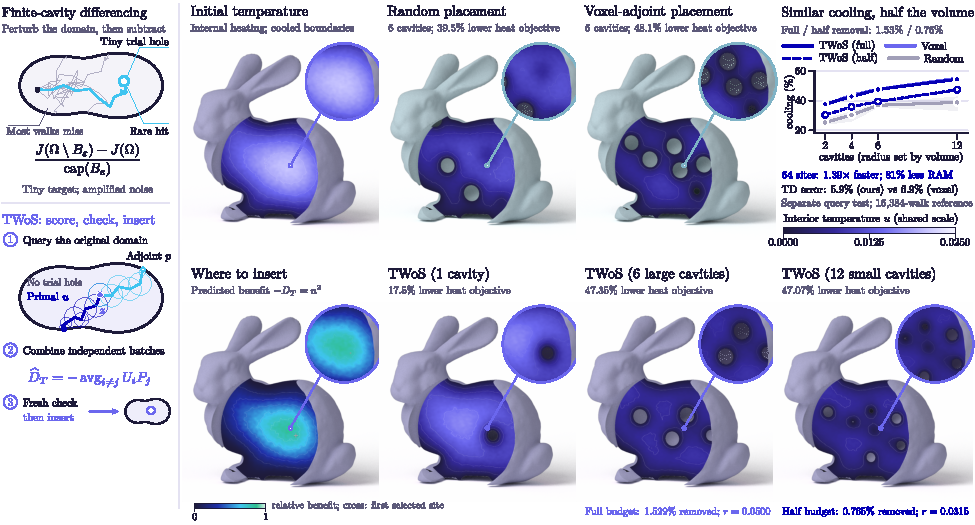
\includegraphics[width=\textwidth]{figures/mesh-hero.pdf}
  \caption{\textbf{Choosing where new cooled cavities should appear.} \method{} queries the current geometry to estimate insertion benefit, then adds selected cavities. Top: initial temperature and six-cavity random and voxel-adjoint designs. Bottom: the initial benefit field, an illustrative first insertion, and two \method{} allocations with similar measured cooling: six large cavities versus twelve small cavities at half the removed volume. These cavities have ideal zero-temperature walls. Temperature views share one color scale; benefit has a separate scale. The cut and inset edges are for display only, and some cavities lie outside the section. Per-design labels use independent objective evaluations; the plot summarizes three design seeds. The speed and memory callouts describe a separate 64-site query benchmark, not the full Bunny optimization. Field rendering and evaluation protocols appear in \cref{sec:bunnybudget,app:renderprotocol}.}
  \label{fig:teaser}
\end{figure}
